Digital image processing is a field of computer vision that deals with the manipulation, analysis, and interpretation of digital images.
It focuses on algorithms and techniques that extract meaningful information from images and enhance visual quality.
We can leverage these algorithms to efficiently and autonomously extract information relevant to model-image registration.

\subsubsection{Filtering and convolution}
\label{sec:filtering-convolution}
As previously discussed, image formation yields a collection of 2D points, $\mathbf{x}_{pix}$.
We can write the intensity values at each pixel location as a digital signal, $f(\mathbf{x}_{pix}) = f(i,j)$, where $(i,j)$ represents the pixel locations in the image, and the function returns the intensity value.
We can then use standard methods of digital signal processing in order to extract meaningful information from images.

The most widely used filter is a linear filter \cite{szeliskiComputerVisionAlgorithms2022}, where the output is some linear operation on the neighboring pixels (\cref{eq:convolution}).
This process is known as a \emph{convolution}.
In a convolution, the kernel, $h$, is shifted along the input image, $f$, and the resultant image, $g$, is the dot product of those two matrices at that specific location.

\begin{equation}
    \begin{aligned}
        g(i,j) &= \sum_{k,l}f(i-k,j-l)h(k,l) \\
        &= \sum_{k,l}f(k,l)h(i-k,j-l) \\
        &\text{Where we use the following notation}\\
        g&= f * h
    \end{aligned}
    \label{eq:convolution}
\end{equation}

The convolution operation is \emph{linear shift invariant}, which means that it obeys the superposition principle (\cref{eq:superposition}) and the shift invariance principle (\cref{eq:shift-invariance}).
This is a powerful property, because it will behave the same everywhere on the input signal/image (e.g. an edge detector will detect an edge, no matter where the edge is on the input image).

\begin{equation}
    h *(f + g) = h*f + h*g
    \label{eq:superposition}
\end{equation}

\begin{equation}
    g(i,j) = f(i+k,j+l) \Longleftrightarrow (h*g)(i,j) = (h*f)(i+k,j+l)
    \label{eq:shift-invariance}
\end{equation}

A common filter applied to images is the Gaussian kernel (\cref{eq:gaussian-kernel}).
This kernel is shaped as a 2D discrete Gaussian, and has the effect of blurring an image and removing noise.

\begin{equation}
    \text{Gaussian filter}=\frac{1}{256}\begin{bmatrix}
        1 & 4 & 6 & 4 & 1 \\
        4 & 16 & 24 & 16 & 4\\
        6 & 24 & 36 & 24 & 6\\
        4 & 16 & 24 & 16 & 4\\
        1 & 4 & 6 & 4 & 1 \\
    \end{bmatrix}
    \label{eq:gaussian-kernel}
\end{equation}

Another is the box kernel, which averages the value of the nearest K pixels (\cref{eq:box-filter}).

\begin{equation}
    \text{Box filter} = \frac{1}{K^{2}}\begin{bmatrix}
        1 & 1 & \cdots &1\\
        1 & 1 & \cdots &1 \\
        \vdots & \vdots & 1 & \vdots \\
        1 & 1 & \cdots & 1
    \end{bmatrix}
    \label{eq:box-filter}
\end{equation}

Edge filters can also be created to detect vertical (\cref{eq:vert-edge-filter}), horizontal (\cref{eq:horiz-edge-filter}), or diagonal edges (\cref{eq:diag-edge-filter}).
As each of the filters moves across the feature it is designed for, that region of the output will be more highly activated than other regions, extracting out the desired components.
The orientation of each of these filters can be hand-selected to find desirable attributes in images.

\begin{equation}
    \text{vertical edge filter} = \begin{bmatrix}
            0 & 1 & 0 \\
            0 & 1 & 0 \\
            0 & 1 & 0 \\
    \end{bmatrix}
    \label{eq:vert-edge-filter}
\end{equation}

\begin{equation}
    \text{horizontal edge filter} =\begin{bmatrix}
        0 & 0 & 0 \\
        1 & 1 & 1 \\
        0 & 0 & 0 \\
    \end{bmatrix}
    \label{eq:horiz-edge-filter}
\end{equation}

\begin{equation}
    \begin{aligned}
        \text{diagonal edge filters} = \begin{bmatrix}
            1 & 0 & 0 \\
            0 & 1 & 0\\
            0 & 0 & 1
        \end{bmatrix}& \text{and} & 
        \begin{bmatrix}
            0 & 0 & 1 \\
            0 & 1 & 0\\
            1 & 0 & 0
        \end{bmatrix}
    \end{aligned}
    \label{eq:diag-edge-filter}
\end{equation}

Lastly, we can use a corner filter to find corners in images (\cref{eq:corner-filter}).

\begin{equation}
    \text{Corner filter} = \frac{1}{4}\begin{bmatrix}
        1 & -2 & 1 \\
        -2 & 4 & -2 \\
        1 & -2 & 1 \\
    \end{bmatrix}
    \label{eq:corner-filter}
\end{equation}

Entire subfields of computer vision and image analysis are devoted to creating increasingly useful and complex filters, or collections of filters. These include steerable filters, which determine information occurring in arbitrary directions \cite{freemanSteerableFiltersLocal1992}, recursive filtering \cite{nielsenRegularizationScalespaceEdge1996}, and non-linear filtering \cite{tomasiBilateralFilteringGray1998}.

\subsubsection{Edge detection}
Edge detection is a highly motivated sub-field of image processing in computer vision due to the immense usefulness of algorithmically determining the edges in a given image.
For a human operator, it can be relatively easy to identify edges of interest, but how can this be achieved computationally?
The first approach might be in viewing an image topographically, with regions of different colors and intensity represented by different ``heights''.
Then, an edge simply becomes an area with a steep gradient (\cref{eq:img-grad}).

\begin{equation}
    \begin{aligned}
        \mathbf{J}(\mathbf{x}) = \nabla I(\mathbf{x}) = (\frac{\partial I}{\partial x}, \frac{\partial I}{\partial y})(\mathbf{x})
    \end{aligned}
    \label{eq:img-grad}
\end{equation}

Finding the direction of the steepest ascent/descent at any given location will give us the normal to the local edge at that point. However, the derivative operator will accentuate and amplify high frequencies in the image, causing noise to overpower the signal. Removing the high-frequency information (a low-pass filter) in the image results in gradient detection that is much more aligned with the salient edges of the image. The Gaussian kernel is a good option for an isotropic low-pass filter on a 2D signal (image) (\cref{eq:gauss-kernel-grad})

\begin{equation}
    \begin{aligned}
        \mathbf{J}_{\sigma}(\mathbf{x}) &= \nabla [G_\sigma (\mathbf{x} * I(\mathbf{x}))] \\
        &= \nabla G_\sigma (\mathbf{x}) * I(\mathbf{x}) \\
        &\text{where} \\
        \nabla G_\sigma (\mathbf{x}) &= (\frac{\partial G_{\sigma}}{\partial x}, \frac{\partial G_{\sigma}}{\partial x}) = [-x - y]\frac{1}{\sigma^{2}}\text{exp}(\frac{-(x^2 + y^2)}{2 \sigma^2})
    \end{aligned}
    \label{eq:gauss-kernel-grad}
\end{equation}


A widely-recognized edge detection algorithm was proposed by John Canny in 1986 \cite{cannyComputationalApproachEdge1986}, and utilizes a five-step process.
First, a Gaussian kernel is applied as a low-pass filter (\cref{eq:gauss-kernel-grad}).
Second, directional filters are used to find the gradients in each direction of the image.
Third, a gradient magnitude threshold is applied to remove noise. Fourth, a double threshold is applied to remove both strong and weak edges.
Last, edges are determined from hysteresis. The prevailing limitation of this algorithm is the need to set kernel size and edge-intensity.

\subsubsection{Binary image processing}
\label{sec:binary-img-proc}

A binary image is a digital image that consists only of black and white pixels.
It is often used for labeling or masking an underlying image, where the values of 1 and 0 represent the presence or absence of a particular feature or object.
Binary images are often used in computer vision and image processing applications due to low computational overhead and quick analysis.
They are also useful for storing and transmitting large amounts of data, as the use of only two values reduces the amount of information that needs to be stored and transmitted.

The primary method of processing binary images is morphological, which involves changing the shape of the ``blob'' in order to extract useful information from it.

\begin{figure}[h!]
    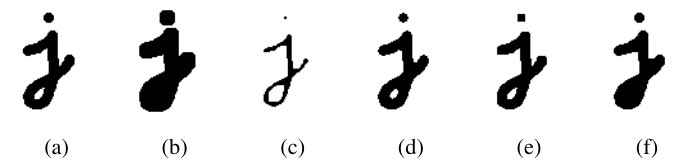
\includegraphics[width = \linewidth]{figs/background/png/binary-image-processing.jpg}
    \caption[A collection of morphological operations on a binary image]{A collection of morphological operations on a binary image: (a) original image; (b) dilation; (c) erosion; (d) majority; (e) opening; (f) closing. Image from \cite{szeliskiComputerVisionAlgorithms2022}}
    \label{fig:binary-image-processing}
\end{figure}

Dilation and erosion are the two main operations that are used in model-image registration (\ref{eq:dilation-erosion}).
These functions are each two-fold: first, a convolution operation is applied to the existing binary image, then a threshold is applied to the convolution output to determine if the central pixel is a 0 or 1.
If $f$ is the input image, $s$ is the convolution kernel of $1$s, and $c=f\otimes s$ is the number of $1$s in the convolution output, then dilation and erosion can be expressed in the following way.

\begin{equation}
    \begin{aligned}
        \text{dilate}(f,s) &= \theta(c,1) \\
        \text{erode}(f,s) &= \theta(c,S) 
    \end{aligned}
    \label{eq:dilation-erosion}
\end{equation}

Where $\theta$ represents a thresholding function.

\begin{equation}
    \theta (f,t) = \begin{cases}
        1 &\text{ if } f\ge t \\
        0 &\text{ else}
    \end{cases}
\end{equation}

%%% Local Variables:
%%% mode: latex
%%% TeX-master: "../../../Andrew_Jensen_Dissertation"
%%% End:
